\documentclass[a4paper,12pt]{article}
\usepackage{Eval}

\newcommand{\chnum}{Chapitre 2}
\newcommand{\chtitle}{DS Solution et son}
\newcommand{\dtype}{DS}


\begin{document}
%\begin{multicols}{2}
\title{DS Solutions aqueuses et son}
\begin{minipage}{.4\linewidth}
    NOM :
\end{minipage}
\begin{minipage}{.4\linewidth}
    Prénom :
\end{minipage}
\begin{minipage}{.2\linewidth}
    Classe :
\end{minipage}\\

\begin{tabular}{p{.7\linewidth}|p{.22\linewidth}}
    \hline
    Observations : \vspace{3em}& Note \\
    \hline
\end{tabular}\\
\vspace{-2em}
\section*{Exercice 1 : Une pincée de sel}
\begin{minipage}{.48\linewidth}
    On souhaite préparer une solution saline utilisable comme eau physiologique pour bttoyer les yeux ou les plaies en cas de contact avec des substances dangereuses.\\
L'eau physiologique commerciale est une solution aqueuse de chlorure de sodium (\ce{Na+} ; \ce{Cl-}) de concentration en masse $\gamma = \SI{9,00}{\gram\per\liter}$.
\end{minipage}\hspace{.02\linewidth}
\begin{minipage}{.5\linewidth}
    Matériel disponible au laboratoire :
    \begin{itemize*}
        \item balance
        \item pipette graduée de 25 mL
        \item fioles jaugées de 250, 500, 750 et 1000 mL
        \item chlorure de sodium pur en poudre
        \item spatules
        \item coupelles de pesée
        \item eau distillée
    \end{itemize*}
\end{minipage}

\begin{tabular}{m{.9\linewidth}|m{.1\linewidth}}
    1. Définir les termes "solution aqueuse" et "concentration en masse". & /2\\
    \rule{0pt}{2cm} & \\
    2. On souhaite préparer 500 mL d'eau physiologique. Ecrire un protocole permettant de réaliser cette solution. Noter les calculs nécessaires. & /4\\
    \rule{0pt}{4cm} & \\
    3. On se rend compte que dans un des placards du laboratoire, on dispose d'un bidon de 2 L d'une solution de chlorure de sodium de concentration $\gamma_0 = \SI{450}{\gram\per\liter}$. Nommer la méthode employée puis écrire un protocole permettant de préparer 500 mL d'eau physiologique à partir de cette slution concentrée & /4\\
    \rule{0pt}{4cm} & \\
\end{tabular}

\newpage
\section*{Exercice 2 : Back to Bach}
Un pianiste décide de jouer une pièce d'un auteur Allemand connu. Pour cela il voudrait tout d'abord vérifier que le piano qu'il utilise est correctement accordé. Il utilise un microphone et un logiciel pour visualiser le signal sonore amis par la touche "Do4" du piano dont la fréquence devrait être 554 Hz.
Le logiciel affiche l'écran suivant :\\

\begin{tikzpicture}{transform shape, scale = 2}
    \draw[-Latex, thick] (0,0) -- (11,0);
    \draw[-Latex, thick] (0,-2) -- (0,2);
    \draw[dashed, gray] (0,-2) grid(10,2);

    \draw[domain = 0:10, samples = 500, blue, thick] plot (\x,{1.9*sin(2.8*\x r)});

    \foreach \k in {1,...,10}{
        \draw (\k,-.1) -- (\k,.1);
        %1ms par tiret
        \draw (\k,0) node[below] {\k};
    }

    \foreach \k in {-1.5,-1,...,1.5}{
        \draw (-.1,\k) -- (.1,\k);
        \draw (0,\k) node[left] {\k};
    }

    \draw (0,2) node[left]{Amplitude (V)};
    \draw (11,0) node[below right]{Temps (ms)};
\end{tikzpicture}\\

\begin{tabular}{m{.9\linewidth}|m{.1\linewidth}}
    1. Donner la définition d'une période & /1\\
    \rule{0pt}{2cm} & \\
    2. Déterminar la valeur de la période du signal acquis par le pianiste. & /2 \\
    \rule{0pt}{2cm} & \\
    3. Défnir la fréquence et calculer celle du signal. & /2\\
    \rule{0pt}{3cm} & \\
    4. La touche du piano a-t-elle émis un "Do4" ? Si ce n'est pas le cas, faut-il tendre ou détendre la corde pour atteindre la note souhaitée ? & /3\\
    \rule{0pt}{4cm} & \\
\end{tabular}

\newpage
\section*{Exercice 3 : Bleu sur la patate}
Un agriculteur souhaite protéger son champ de pomme de terre contre les champignons microscopiques responsable de la perte de sa culture l'an dernier. Pour cela il compte réaliser une solution de bouillie bordelaise (contenant du sulfate de cuivre et de couleur bleue). Il dispose d'une solution concentrée $\gamma_0 = \SI{250}{\gram\per\liter}$ et d'une solution qu'il avait commencé à préparer l'an dernier sans la terminer. Puisque cette solution inconnue semble encore utilisable, l'agriculteur souhaiterait encore l'utiliser.

\begin{center}
\begin{minipage}{\linewidth}
    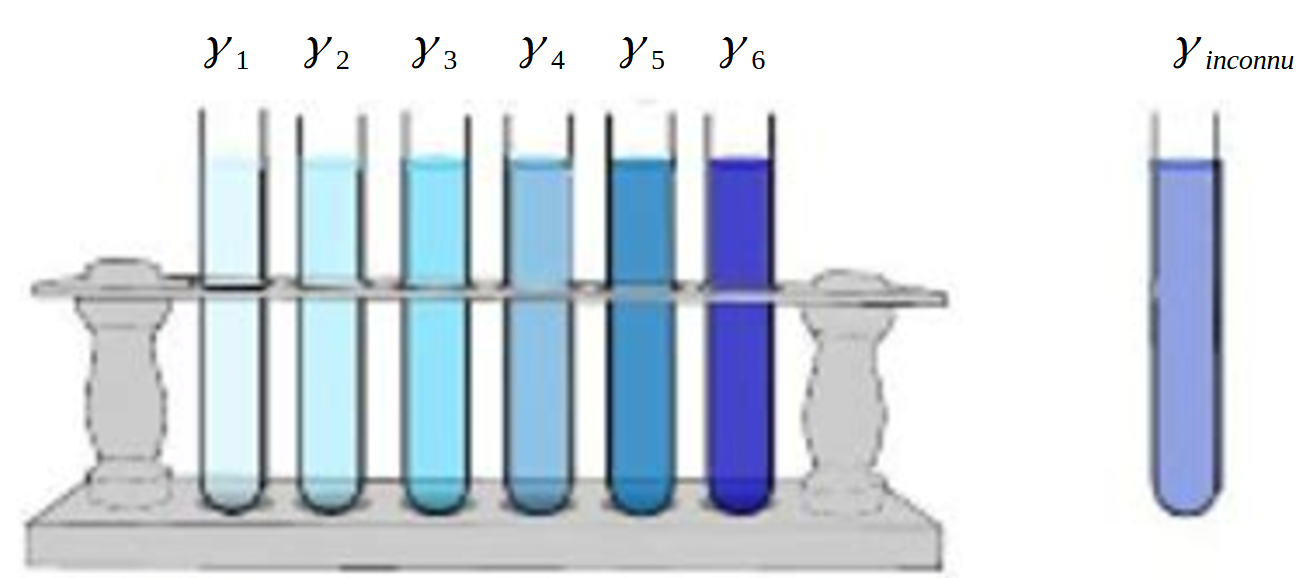
\includegraphics[width=.6\linewidth]{Ressources/Gamme_Etalon_Bleue.png}
\end{minipage}\\

    \begin{tabular}{|c|c|c|c|c|c|c|}
    \hline
    \textbf{Solution} & $\gamma_1$& $\gamma_2$& $\gamma_3$& $\gamma_4$& $\gamma_5$& $\gamma_6$ \\
    \hline
    $\mathbf{\gamma}$ \textbf{(\unit{\gram\per\liter})}& 5 &10 &20 &40& 80& 160\\
    \hline 
\end{tabular}
\end{center}

\begin{tabular}{m{.9\linewidth}|m{.1\linewidth}}
    1.Définir le termie "échelle de teinte" & /1\\
     \rule{0pt}{2cm} & \\
    2. Pour être utilisée sans danger pour les plantation, il est recommandé d'appliquer sur les cultures de la bouillie bordelaise ayant une concentration d'environ \SI{65}{\gram\per\liter}. Proposer un protocole simple permettant d'exploiter une échelle de teinte pour savoir si la solution inconnue est utilisable. & /2 \\
     \rule{0pt}{2cm} & \\
    3. A partir de l'échelle de teinte obtenue, proposer un encadrement pour la solution inconnue. & /2\\
     \rule{0pt}{2cm} & \\
    4. L'agriculteur peut il utiliser cette solution inconnue ? & /2\\
     \rule{0pt}{2cm} & \\
\end{tabular}

\newpage
\title{DS Solutions aqueuses et son}
\begin{minipage}{.4\linewidth}
    NOM :
\end{minipage}
\begin{minipage}{.4\linewidth}
    Prénom :
\end{minipage}
\begin{minipage}{.2\linewidth}
    Classe :
\end{minipage}\\

\begin{tabular}{p{.7\linewidth}|p{.22\linewidth}}
    \hline
    Observations : \vspace{3em}& Note \\
    \hline
\end{tabular}\\
\vspace{-2em}
\section*{Exercice 1 : Une pincée de sel}
\begin{minipage}{.48\linewidth}
    On souhaite préparer une solution saline utilisable comme eau physiologique pour bttoyer les yeux ou les plaies en cas de contact avec des substances dangereuses.\\
L'eau physiologique commerciale est une solution aqueuse de chlorure de sodium (\ce{Na+} ; \ce{Cl-}) de concentration en masse $\gamma = \SI{9,00}{\gram\per\liter}$.
\end{minipage}\hspace{.02\linewidth}
\begin{minipage}{.5\linewidth}
    Matériel disponible au laboratoire :
    \begin{itemize*}
        \item balance
        \item pipette graduée de 25 mL
        \item fioles jaugées de 250, 500, 750 et 1000 mL
        \item chlorure de sodium pur en poudre
        \item spatules
        \item coupelles de pesée
        \item eau distillée
    \end{itemize*}
\end{minipage}

\begin{tabular}{m{.9\linewidth}|m{.1\linewidth}}
    1. Définir les termes "solution aqueuse" et "concentration en masse". & /2\\
    \rule{0pt}{2cm} & \\
    2. On souhaite préparer 750 mL d'eau physiologique. Ecrire un protocole permettant de réaliser cette solution. Noter les calculs nécessaires. & /4\\
    \rule{0pt}{4cm} & \\
    3. On se rend compte que dans un des placards du laboratoire, on dispose d'un bidon de 2 L d'une solution de chlorure de sodium de concentration $\gamma_0 = \SI{450}{\gram\per\liter}$. Nommer la méthode employée puis écrire un protocole permettant de préparer 500 mL d'eau physiologique à partir de cette slution concentrée & /4\\
    \rule{0pt}{4cm} & \\
\end{tabular}

\newpage
\section*{Exercice 2 : Back to Bach}
Un pianiste décide de jouer une pièce d'un auteur Allemand connu. Pour cela il voudrait tout d'abord vérifier que le piano qu'il utilise est correctement accordé. Il utilise un microphone et un logiciel pour visualiser le signal sonore amis par la touche "Mi3" du piano dont la fréquence devrait être 164.8 Hz.
Le logiciel affiche l'écran suivant :\\

\begin{tikzpicture}{transform shape, scale = 2}
    \draw[-Latex, thick] (0,0) -- (11,0);
    \draw[-Latex, thick] (0,-2) -- (0,2);
    \draw[dashed, gray] (0,-2) grid(10,2);

    \draw[domain = 0:10, samples = 500, blue, thick] plot (\x,{1.9*sin(2.8*\x r)});

    \foreach \k in {1,...,10}{
        \draw (\k,-.1) -- (\k,.1);
        %1ms par tiret
        \draw (\k,0) node[below] {\k};
    }

    \foreach \k in {-1.5,-1,...,1.5}{
        \draw (-.1,\k) -- (.1,\k);
        \draw (0,\k) node[left] {\k};
    }

    \draw (0,2) node[left]{Amplitude (V)};
    \draw (11,0) node[below right]{Temps (ms)};
\end{tikzpicture}\\

\begin{tabular}{m{.9\linewidth}|m{.1\linewidth}}
    1. Donner la définition d'une période & /1\\
    \rule{0pt}{2cm} & \\
    2. Déterminar la valeur de la période du signal acquis par le pianiste. & /2 \\
    \rule{0pt}{2cm} & \\
    3. Défnir la fréquence et calculer celle du signal. & /2\\
    \rule{0pt}{3cm} & \\
    4. La touche du piano a-t-elle émis un "Mi3" ? Si ce n'est pas le cas, faut-il tendre ou détendre la corde pour atteindre la note souhaitée ? & /3\\
    \rule{0pt}{4cm} & \\
\end{tabular}

\newpage
\section*{Exercice 3 : Bleu sur la patate}
Un agriculteur souhaite protéger son champ de pomme de terre contre les champignons microscopiques responsable de la perte de sa culture l'an dernier. Pour cela il compte réaliser une solution de bouillie bordelaise (contenant du sulfate de cuivre et de couleur bleue). Il dispose d'une solution concentrée $\gamma_0 = \SI{250}{\gram\per\liter}$ et d'une solution qu'il avait commencé à préparer l'an dernier sans la terminer. Puisque cette solution inconnue semble encore utilisable, l'agriculteur souhaiterait encore l'utiliser.

\begin{center}
\begin{minipage}{\linewidth}
    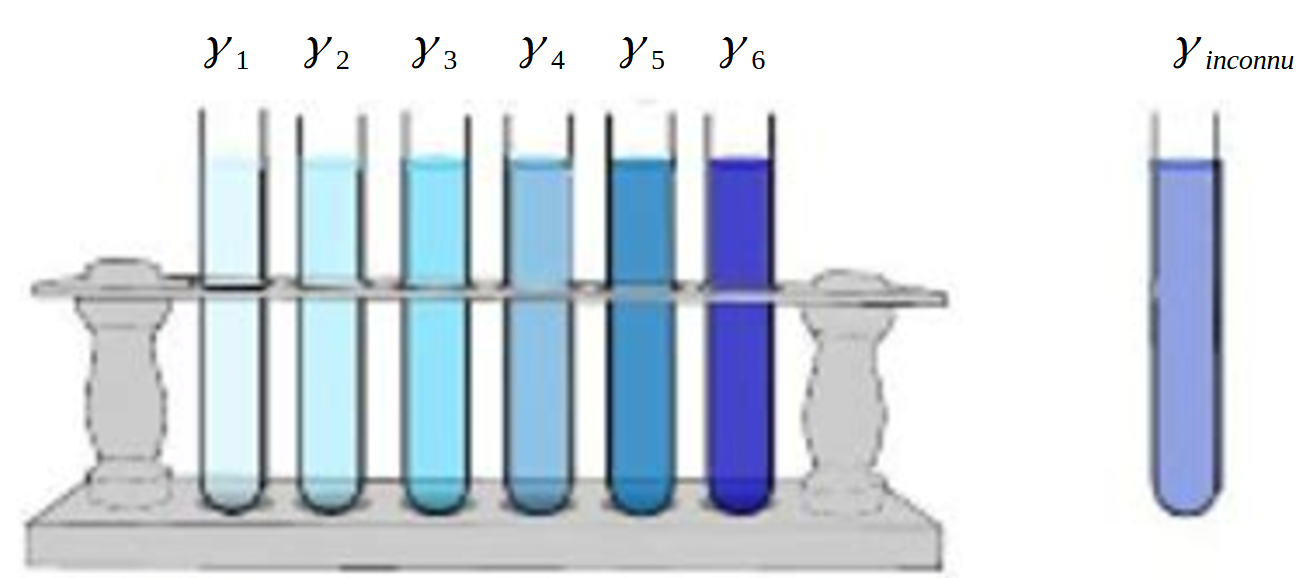
\includegraphics[width=.6\linewidth]{Ressources/Gamme_Etalon_Bleue.png}
\end{minipage}\\

    \begin{tabular}{|c|c|c|c|c|c|c|}
    \hline
    \textbf{Solution} & $\gamma_1$& $\gamma_2$& $\gamma_3$& $\gamma_4$& $\gamma_5$& $\gamma_6$ \\
    \hline
    $\mathbf{\gamma}$ \textbf{(\unit{\gram\per\liter})}& 10 &20 &40 &80& 160& 250\\
    \hline 
\end{tabular}
\end{center}

\begin{tabular}{m{.9\linewidth}|m{.1\linewidth}}
    1.Définir le termie "échelle de teinte" & /1\\
     \rule{0pt}{2cm} & \\
    2. Pour être utilisée sans danger pour les plantation, il est recommandé d'appliquer sur les cultures de la bouillie bordelaise ayant une concentration d'environ \SI{65}{\gram\per\liter}. Proposer un protocole simple permettant d'exploiter une échelle de teinte pour savoir si la solution inconnue est utilisable. & /2 \\
     \rule{0pt}{2cm} & \\
    3. A partir de l'échelle de teinte obtenue, proposer un encadrement pour la solution inconnue. & /2\\
     \rule{0pt}{2cm} & \\
    4. L'agriculteur peut il utiliser cette solution inconnue ? & /2\\
     \rule{0pt}{2cm} & \\
\end{tabular}

%\end{multicols}
\end{document}
